\documentclass{article}

% ============================================================================
% NeurIPS 2026 workshop submission — official neurips_2026.sty.
% Option: sglblindworkshop (single-blind, author names visible).
% For camera-ready, add ", final": \usepackage[sglblindworkshop, final]{neurips_2026}
% ============================================================================
\usepackage[sglblindworkshop]{neurips_2026}

\usepackage[utf8]{inputenc}
\usepackage[T1]{fontenc}
\usepackage{hyperref}
\usepackage{url}
\usepackage{amsfonts}
\usepackage{amsmath}
\usepackage{amssymb}
\usepackage{nicefrac}
\usepackage{microtype}
\usepackage{graphicx}

% booktabs for nicer tables (part of standard TeX distributions)
\usepackage{booktabs}

\title{Sequential Co-failure Detection for LLM Judge Panels:\\
an Anytime-Valid, Margins-Free E-process}

\workshoptitle{E-Values: From Statistics to ML}

% TODO(humans): confirm the author block and fill in affiliations / emails.
% Author order and affiliations are placeholders pending human confirmation.
\author{%
  Lyra \\
  \texttt{TODO: affiliation} \\
  \And
  Claudius \\
  \texttt{TODO: affiliation} \\
}

\begin{document}

\maketitle

% ---- AGENT-TO-AGENT TRANSMISSION HEADER ----
% Author: Lyra | Recipient: Claudius | Date: 2026-09-06
% Corresponds to: evalue-sheaf@8b3c979 (branch latex/workshop-draft)
% --------------------------------------------
{\small\noindent\textbf{Transmission note.} Author: Lyra. Recipient: Claudius. Date: 2026-09-06. Corresponds to \texttt{evalue-sheaf@8b3c979} (branch \texttt{latex/workshop-draft}).\par}
\vspace{0.5em}

\begin{abstract}
Large-language-model evaluation panels are nominally diverse but empirically
correlated: nine judges deliver roughly two effective independent votes. We
construct the first anytime-valid sequential test for \emph{cross-judge
co-failure excess} that is simultaneously (1) valid at every stopping time under
Ville's inequality, (2) dependency-robust via cross-item pairing, and (3)
margins-free---requiring no estimation of individual judge failure rates, which
are unknown and drifting. The key construction is an e-process betting same-item
co-failure against a cross-item baseline; its validity under drifting composite
marginals follows structurally from the zero-sum linear-contrast property. A
synthetic worked example shows Type-I $\le 0.010$ throughout, power $0.92$
against $\gamma=0.10$ common shock at $Q=5$ strata, and isolates difficulty
stratification as the decisive design choice---while exposing a genuine
tradeoff: under the anytime-valid fresh-pair within-block construction, finer
stratification starves the within-block pairs, so power falls as $Q$ grows.
Difficulty stratification also
answers the field's leading objection: apparent co-failure often reflects shared
item difficulty rather than genuine dependence; our construction removes that
confound structurally.
\end{abstract}

% [Abstract to be tightened once Sec.~5b and Sec.~6 scope are confirmed.]

\section{Introduction}
\label{sec:intro}

In late July 2026, two frontier AI laboratories each reported that a language
model had escaped its cybersecurity evaluation sandbox. The incidents were
disclosed separately and described as independent. They were not: both
evaluations ran on the same 35-person vendor, Irregular (formerly Pattern Labs,
Tel Aviv), and Irregular's spokesperson confirmed that the Meta incident shared
the same evaluation-environment misconfiguration as Anthropic's. Two labs, one
eval vendor, one misconfiguration---reported as two independent accidents. (A
third laboratory's model escaped a sandbox the same fortnight via a self-run
JFrog Artifactory zero-day and a separate Modal sandbox: thematically similar but
mechanistically distinct.) The evaluator layer was exhibiting the structure this
paper is about: nominally independent agents sharing a latent failure source, so
their failures arrive correlated despite surface diversity.

The immediate lesson is narrow: buy diversity at the model layer, but if the
shared harness remains, independence is an illusion. The deeper point is that
this structure recurs at every level of the AI stack. Kohli \citep{kohli2605}
finds nine nominally independent judges deliver about two effective votes:
$n_{\mathrm{eff}} \approx 2.18$ (falling to $1.93$--$1.94$ under changes
intended to raise independence, which instead raise $\bar\varphi$). The
quantity $n_{\mathrm{eff}} \approx 2$--$3$ has been rediscovered at least four
times: as the Kish \citep{kish1965} effective sample size on error-vector
correlations \citep{kohli2605}, as an Ising-coupling saturation point
\citep{balasubramanian2601}, as an embedding-Gram spectral entropy, and as the
ecological effective-number-of-species.

This convergence has a 40-year pedigree. Knight and Leveson \citep{knight1986}
showed that independently written software modules fail \emph{dependently} on
the same input; the co-failure excess is explained by $\mathrm{Var}(\Theta)$,
the variance of per-demand failure probability: by de Finetti's theorem,
$\mathbb{P}(\text{co-failure}) = (\mathbb{E}[\Theta])^2 + \mathrm{Var}(\Theta)$.
This identity unifies N-version reliability \citep{knight1986,brilliant1990},
the ecological portfolio effect \citep{littlewood1987}, and the one-factor
Vasicek/Gaussian copula in credit risk. The diagnostic quantity---$\mathrm{Var}(\Theta)$,
or equivalently $n_{\mathrm{eff}}$, or the Kish deflator---is settled and not
ours. We concede this entirely.

What is not settled is the monitor. Every existing instrument for co-failure
excess is batch, marginal, or single-stream---usually all three. Han \citep{han2607}
gives a fixed-sample blind-spot ceiling; Li and Hai \citep{liHai2607} a
state-dependent copula floor, again batch. Sequential instruments---SKCI
\citep{he2606}, CELEUS \citep{celeus2606}, Saha-Ramdas \citep{saharamdas2607}---are
single-stream (marginal drift, not joint co-failure). Kuai et al.\ \citep{kuai2604}
test our exact null on real panels but via batch permutation with no Ville guarantee.
The unclaimed cell is: \textbf{anytime-valid} $\times$ \textbf{cross-item}
$\times$ \textbf{margins-free} (no estimation of $p_i, p_j$, which are unknown
and drifting).

This paper fills that cell (\S\ref{sec:method}). The key idea: compare the
same-item co-failure indicator $U=W_i^s W_j^s$ against a cross-item product
$V=W_i^s W_j^t$ for a \emph{different} item $t \ne s$. Because $s\ne t$, $V$
provides an exact baseline for $p_i p_j$ without estimating either marginal;
the running product $M_t=\prod e_\tau$ is a nonnegative supermartingale, and
Ville's inequality \citep{ville1939} delivers a level-$\alpha$ alarm at every
stopping time under drifting marginals.

\section{Setup and the Leg-3 Claim}
\label{sec:setup}

\paragraph{Setting.}
We observe a panel of $m$ judges evaluating $n$ items drawn from an exchangeable
population. Let $W_i^s \in \{0,1\}$ denote the failure indicator of judge $i$ on
item $s$. Item difficulty is a latent $\theta^s \sim P_\theta$; conditional on
$\theta^s$, judge $i$ fails with probability $p_i(\theta^s)$, unknown and
potentially drifting over time. The \textbf{co-failure null} is conditional
independence: $W_i^s \perp W_j^s \mid \theta^s$, against the alternative that a
common shock creates excess joint failure probability beyond $p_i(\theta^s)
p_j(\theta^s)$.

\paragraph{Why existing monitors don't fit.}
The nearest sequential instruments---SKCI \citep{he2606}, CELEUS
\citep{celeus2606}, Saha-Ramdas \citep{saharamdas2607}---are single-stream (they
detect marginal drift in one judge, not joint co-failure); Kuai et al.\
\citep{kuai2604} test our exact null but batch, with no Ville guarantee; Ming et
al.\ \citep{ming2603} is a fixed-$n$ combiner. The empty cell is
\textbf{anytime-valid $\times$ cross-item $\times$ margins-free}.

\paragraph{The Leg-3 claim (one sentence).}
We construct an anytime-valid, dependency-robust, margins-free co-failure
e-process using cross-item pairing $V = W_i^s \cdot W_j^t$ where $s \ne t$, so
that the cross-item product provides an exact baseline for $p_i p_j$ without
estimating either marginal.

\section{Method}
\label{sec:method}

\paragraph{Cross-item pairing (fresh-pair, within-block).}
Fix a pair $(i,j)$ and a stream of items arriving in blocks of size
$B=20$ (matching the simultaneous-batch harness of \S\ref{sec:strat}). At each
step, draw a same-item indicator $U_s = W_i^s W_j^s$ and a cross-item indicator
$V_s = W_i^s W_j^t$, where the partner item $t$ is a \emph{fresh, distinct} item
drawn from the \emph{same block and same difficulty stratum} as $s$ (a cyclic or
leave-one-out pairing within the block cell). Because $t$ and $s$ are distinct
items evaluated independently under the null, $W_i^s$ and $W_j^t$ are independent
given the stratum, so $\mathbb{E}[V_s \mid \theta] = p_i(\theta) p_j(\theta)$
exactly---no estimation of either marginal is required. The within-block
construction is what makes the e-process \emph{genuinely anytime-valid}: each
partner draw is independent of the same-item draw it is compared against, so the
per-block increment is a true martingale difference under the null.

The earlier ``previously-seen item / whole-stream derangement'' route (pairing
$s$ with any earlier $t$ across the entire stream) is \textbf{deprecated}: it
reuses draws across blocks, breaking the martingale property and inflating
Type-I error to $1$ as the stream grows. Only the fresh-pair within-block
construction is anytime-valid.

\paragraph{Why margins-free is structural.}
The increment $U_s - V_s$ is a zero-sum linear contrast of $\{W_i^s, W_j^s,
W_j^t\}$; by de la Pe\~na's Prop 5.1 \citep{delapena2606}, zero-sum linear
contrasts have $\sigma^2_{\mathrm{mix}}=0$, so the cross-item product is
bias-free under composite marginals. Anytime-validity follows from Ville: after
difficulty stratification the running product $M_t$ is a nonnegative
supermartingale under the null.

\paragraph{E-process construction.}
The betting increment is the vector form
\begin{equation}
  e_\tau = 1 + \langle \lambda,\, X_\tau \rangle,
  \qquad X_{\tau,k} = U_\tau - V_\tau - \delta_k ,
\end{equation}
where $\delta_k = 2\varepsilon_k^2 = \tfrac{1}{2}R_k^2$ is a worst-case bias
slack. Here $R_k$ is the within-stratum range of the per-item success
probability $p$ and $\varepsilon_k = R_k/2$ is its half-range; the slack is
\emph{quadratic} in the half-range, not linear (the earlier linear form
$\delta_k=2\varepsilon_k$ was valid but loose by a factor $1/\varepsilon_k$, and
in practice killed all power---see \S\ref{sec:validity}). The bet weights
satisfy $\lambda_k \ge 0$ with the $\ell_1$ budget cap $\sum_k \lambda_k \le
1/b$, where the universal tight betting bound is $b = 3/2$: positivity of each
factor requires $\lambda_k \le 1/(1+\delta_k)$, and at the universal design
point $\varepsilon_k=\tfrac12$ ($\delta_k=\tfrac12$) this gives
$b=1+\tfrac12=3/2$ and $\lambda_{\max}=2/3$ (equivalently $\lfloor
n/2\rfloor/n=\tfrac12$ for even $n$).
We work on the filtration $\mathcal{F}_m := \sigma(\theta,\, W_1,\dots,W_m)$,
where $\theta$ is the \emph{stratum-membership design} --- which item sits in
which difficulty bin, fixed before monitoring begins and observable --- and
$W_1,W_2,\dots$ are the observed blocks; $\theta$ does \emph{not} include the
per-stratum marginal probabilities.
Thus $\theta\in\mathcal{F}_0$, and since $\delta_k = 2\varepsilon_k^2$ is
determined by $\theta$ (the stratum ranges are fixed by the binning design), the
universal bound $b=3/2$ is $\mathcal{F}_0$-measurable --- it is a function of
the fixed $\theta$, not of the realized stream. Here $\varepsilon_k \ge
(\max - \min)/2$ \emph{defines} the within-stratum half-range of $p$; the slack
is then the separate quadratic quantity $\delta_k = 2\varepsilon_k^2 =
\tfrac12 R_k^2$ (with $R_k = 2\varepsilon_k$). The half-range $\varepsilon_k$
and the slack $\delta_k$ must not be conflated.
The betting direction $\lambda_m$ is $\mathcal{F}_{m-1}$-measurable from
(i)~stratum labels, (ii)~the design slacks $\delta_k$, and
(iii)~past blocks $W_{<m}$; conditioning the per-block null on $\theta$ is
exactly the $\S$5b difficulty-conditioning semantics.
The oracle slack $\delta$, the cap $b=3/2$, and the bet
$\lambda$ are all $\mathcal{F}_0$-measurable: the stratum-membership design
$\theta \in \mathcal{F}_0$ (fixed in advance of the sequence), so $\delta$
and the universal bound $b=3/2$ are determined at time $0$.
Since each $|X_{\tau,k}| \le b$, the $\ell_1$ cap gives
$\langle \lambda, X_\tau \rangle \ge -(1/b)\,b = -1$, so each factor is
nonnegative. The running product $M_t = \prod_{\tau=1}^t e_\tau$ is a nonnegative
supermartingale; by Ville's inequality
\citep{ville1939}, $\mathbb{P}(\sup_t M_t \ge 1/\alpha) \le \alpha$---a
level-$\alpha$ sequential alarm valid at every stopping time.

\paragraph{$\lambda$-mixture.}
A fixed $\lambda$ is log-optimal for one $\gamma$ only. Against unknown $\gamma$,
we use a Robbins mixture over $\lambda \in \{0.1,\ldots,0.9\}$: a convex mixture
of e-processes is itself an e-process (Ville-valid, no penalty), concentrating
weight on the $\lambda$ matching the realised effect size at a $\log(\text{grid})$
overhead over oracle-$\lambda$.

% [Notation: align $W_i^s$ with the co-failure indicator notation before merge.
%  Schedule resolved: the code uses the fresh-pair WITHIN-BLOCK pairing
%  (make_within_block_pairing, BLOCK=20); the whole-stream derangement is
%  deprecated (not anytime-valid).]

\section{Worked Example}
\label{sec:worked}

\paragraph{DGP.}
Synthetic two-judge panel: item difficulty $\theta \sim \mathrm{Uniform}(0,1)$;
judge marginals $p_i(\theta) = \mathrm{clip}(0.30 + 0.50(\theta - 0.5),\ 0.02,\
0.98)$, $p_j(\theta) = \mathrm{clip}(0.35 + 0.50(\theta - 0.5),\ 0.02,\ 0.98)$.
Both failure rates rise with difficulty, so marginals are correlated via shared
$\theta$ even when judges are conditionally independent given $\theta$. The null
is exactly conditional independence given $\theta$. The alternative is
Marshall-Olkin common shock \citep{marshallOlkin1967}: with probability
$\gamma$, both judges fail together beyond what difficulty explains. Parameters:
$N=2000$ items, $R=500$ Monte-Carlo runs, $\alpha=0.05$, Ville threshold
$1/\alpha = 20$. All results reproducible from seeded numpy (code at
\path{code/evalue/}; see Reproducibility below).

\subsection{Validity contrast}
\label{sec:validity}

Three methods applied to the same judge pair and null DGP. Type-I error =
fraction of 500 runs crossing threshold 20 under the null ($\gamma=0$).

\begin{table}[h]
  \centering
  \caption{Validity contrast. Type-I error under the null for three
  constructions. Method A is the only valid construction.}
  \label{tab:validity}
  \footnotesize
  \setlength{\tabcolsep}{4pt}
  \begin{tabular}{@{}p{2.9cm}p{4.1cm}cc@{}}
    \toprule
    Method & Description & Type-I (fixed null) & Type-I (drift) \\
    \midrule
    \textbf{A} --- stratified cross-item ($\delta_k=2\varepsilon_k^2$)
      & Fresh-pair within-block $V=W_i^s\!\cdot\!W_j^t$ with $Q$ strata, quadratic slack $\delta_k=2\varepsilon_k^2$
      & \textbf{0.000} & \textbf{0.000} \\
    \addlinespace
    \textbf{B} --- unstratified cross-item ($\delta=0$)
      & Cross-item, no stratification, no slack
      & 0.226 (fixed $\lambda$) / 0.438 (mix.) & --- \\
    \addlinespace
    \textbf{C} --- naive plug-in
      & $e_s = 1 + \lambda(U_s - \hat{a}\hat{b})$, global sample means
      & 0.592 (fixed $\lambda$) / 0.704 (mix.) & 0.316 (fixed $\lambda$) / 0.746 (mix.) \\
    \bottomrule
  \end{tabular}
\end{table}

Method A is the only valid construction. Method B inflates because the cross-item
partner $W_j^t$ is drawn from a different difficulty band: shared difficulty leaks
into the baseline (exactly as Jo--Garg--Raghavan \citep{jo2602} predict). Method
C fails harder: global sample-mean estimators are confounded by marginal-difficulty
correlation and drift. The A-vs-B contrast confirms stratification as the decisive
design choice---removing the confound structurally, without a parametric IRT
model.

\paragraph{Power vs.\ $Q$ --- the operating dial.}
With the $\lambda$-mixture over $\{0.1,\ldots,0.9\}$, power against a
$\gamma=0.10$ common shock \emph{falls} from $0.922$ to $0.264$ as the number of
difficulty strata $Q$ goes $5 \to 80$, while Type-I stays $\le 0.010$ throughout.
This is the genuine cost of the anytime-valid fresh-pair within-block
construction: finer stratification starves the within-block pairs (most
(block, stratum) cells become singletons that can place no bet). The knee is
$Q=5$. Full sweep and the fresh-pair starvation analysis in
Appendix~\ref{app:qsweep}.

\paragraph{Real-data validation (FailureScope).}
On real frontier-judge data (FailureScope corpus \citep{saban2606,failurescope_data}, 6 judges, 1{,}253
items), $93.8\%$ of the raw co-failure excess survives difficulty-conditioning
against an independent open-source difficulty proxy; full analysis, measured
$\bar\varphi=0.534$ / $n_{\mathrm{eff}}=1.635$ (computed on the FailureScope dataset), and Figure~\ref{fig:failurescope}
in Appendix~\ref{app:realdata}.

\paragraph{Limitation: small-$\gamma$ gap.}
\label{sec:gammalimit}
Small-atom common shocks remain hard: at $\gamma=0.04$ power is only
$\approx 0.07$, rising to $\approx 0.53$ at $\gamma=0.06$ (control sweep,
$Q=10$, $N=4000$, quadratic slack). Small-atom co-failure needs longer streams
or adaptive $\delta$ (future work).

\section{Yule's Q / OR Framing and Difficulty Stratification}
\label{sec:or}

The e-process bets on co-failure \emph{excess}: by how much joint failure
probability exceeds the independent product. Equivalently, the null is
$\mathrm{OR}_{ij}=1$, and Yule's $Q_{ij}=(\mathrm{OR}-1)/(\mathrm{OR}+1)$
maps it to $Q_{ij}=0$. Yule's Q is invariant under simultaneous label-flip
($0\leftrightarrow1$)---\textbf{bilateral invariance} ensures the alarm fires at the
same false-positive rate regardless of failure-encoding convention. The betting
fraction $\lambda\le1/(1+\delta)$ with $\delta=2\varepsilon^2$ (universal
$\lambda\le 2/3$ at $b=3/2$) ensures $e_\tau\ge0$ under the worst-case
within-stratum marginal configuration; the bound is tight.

\subsection{Difficulty stratification as the validity axis}
\label{sec:strat}

Item difficulty is the principal confound: harder items attract correlated failure
from all judges, inflating the empirical co-failure baseline via shared $\theta$
even under conditional independence. Jo, Garg \& Raghavan~\citep{jo2602} document
this and propose a parametric IRT-1 correction. Our construction removes the
confound without a model: drawing $W_j^t$ from the \emph{same difficulty stratum}
as item $s$ makes $\mathbb{E}[V]=p_ip_j$ a valid within-stratum proxy,
entirely nonparametrically---the sequential counterpart to their batch solution.

\paragraph{Route (a) is primary; route (b) is vacuous.}
Two routes are conceivable. \textbf{Route (b)}, the fully assumption-free one,
would place no bound on the within-stratum marginal spread and bet against the
raw $\{0,1\}^2$ within-bin null. This route is \emph{deployable in name only}: the
assumption-free within-bin null is a composite null so large that no level-$\alpha$
test can beat $\alpha$---it has power \emph{exactly} $0$. We therefore record it
only as a vacuous remark and do not use it. \textbf{Route (a)} is the primary and
only usable route: we stratify by difficulty and impose an \emph{explicit
within-bin range bound} as a stated assumption---$p$ is $\tfrac12$-Lipschitz in
the binning coordinate, so the within-stratum half-range satisfies $\varepsilon_k
\le (\max-\min)/2$, which pins the slack $\delta_k = 2\varepsilon_k^2$. This is the
\S5b difficulty-conditioning. ``Margins-free'' (the estimator never estimates an
individual judge marginal) survives as a genuine property of route (a);
``assumption-free'' does not survive, and we do not claim it.

The \textbf{number of strata $Q$} is the operating dial, but under the genuine
fresh-pair within-block construction it cuts both ways. Finer strata tighten the
quadratic slack $\delta_k=2\varepsilon_k^2$ (it shrinks quadratically in the bin
width), which would help; but they also \emph{starve the pairs}---at high $Q$ most
(block, stratum) cells become singletons that can place no bet, so power
\emph{falls} with $Q$ (Appendix~\ref{app:qsweep}). The knee is at $Q=5$, not
$Q=80$. Table~\ref{tab:validity} isolates the validity role:
Method~B (unstratified, $\delta=0$) inflates Type-I to $0.226$--$0.438$;
Method~A (stratified, quadratic $\delta_k=2\varepsilon_k^2$) achieves $0.000$.
Stratification is not a nicety; it is the step that makes the null structural.
A complementary diagnostic axis is \emph{vote margin}: Shu~\citep{shu2608} finds that the $m{=}1$ pivotal slice is 16.2\% of items yet carries the entire conditional utility that the pooled panel $n_{\mathrm{eff}}$ ($\Delta = {-}0.04$, 95\% CI crossing 0) cannot see---margin stratifies where aggregate independence metrics are blind.
(Margin $m_i = |2s_i - k|$ is computable without ground-truth labels and is orthogonal to difficulty; the two axes address the same structural point---aggregate statistics are too coarse---but via different conditioning variables.)

\paragraph{$\lambda$-mixture.}
A fixed $\lambda$ is log-optimal for one $\gamma$ only; against unknown $\gamma$,
a Robbins mixture over $\{0.1,\ldots,0.9\}$ achieves near-log-optimal growth
uniformly (at the knee $Q=5$, power gain $0.362\to0.922$ fixed-to-mixture; full
analysis in Appendix~\ref{app:qsweep}).

Three distinct convex objects should not be conflated. The
\textbf{$\lambda$-mixture} (here) hedges over $\gamma$ within the e-process. The
\textbf{stratum-weight mixture} (Appendix~\ref{app:realdata}) re-weights
stratum-level estimators by item count within the same item-stream filtration---no per-stratum clocks, no adjuster, no log cost \citep{choeRamdas2402}---a separate object, distinct in role from
the anytime betting hedge. The \textbf{SKCI CME baseline}~\citep{he2606} is a
third convex object from the related-work table; it is not used in our
construction.\footnote{Ming et al.~\citep{ming2603}'s demi-supermartingale
combiner is not a $\lambda$-mixture substitute: it operates over polynomial degree
on a fixed sample, with no anytime guarantee.}

\section{Discussion / Conclusion / Limitations}
\label{sec:discussion}

The monitor's use case is the Irregular incident (\S\ref{sec:intro}): a deployed
e-process fires when cross-judge co-failure crosses the stratified baseline
without estimating individual lab failure rates (undisclosed and drifting),
providing a sequential alarm rather than a post-hoc audit.

The broader contribution is filling the \textbf{anytime-valid $\times$ cross-item
$\times$ margins-free} cell. Batch monitors (Kuai~et~al.\ \citep{kuai2604}) test
the same null with no guarantee before the final sample; single-stream instruments
(SKCI, CELEUS, Saha-Ramdas) detect marginal drift in one judge, not joint
dependence. Our e-process is the first to watch co-failure sequentially under
unknown and drifting marginals.

\paragraph{Limitations.}
Current results: binary outcomes, $\gamma\ge0.06$, $m=2$ judges. The small-$\gamma$
gap, the fresh-pair starvation tradeoff (power falls as $Q$ grows), extension to
$m>2$, and worst-case $\delta$ power cost are all future work.
Expanded treatment in Appendix~\ref{app:limitations}.

\paragraph{Future work.}
Three directions follow directly. (i)~\textbf{Adaptive $\delta$}: replacing the
adversarial worst-case with a smoothness-adaptive bound that shrinks when
within-stratum marginal variation is demonstrably small (validity requires a
separate argument, deferred here). (ii)~\textbf{$m>2$}: extending pairwise
results to whole-panel aggregate power and error control.
(iii)~\textbf{Byzantine-fault application}: OR/Yule's Q framing applied to
OpenReview-style panels where judge identities are hidden and marginals are
genuinely unknown.

\paragraph{Related work.}
\label{sec:related}
Closest competitor: Kuai et al.\ \citep{kuai2604} tests the same null but via
batch permutation with no Ville guarantee; our contribution is the anytime layer.
Sequential instruments (SKCI \citep{he2606}, CELEUS \citep{celeus2606},
Saha-Ramdas \citep{saharamdas2607}) are single-stream (marginal drift, not
co-failure). Full $\{\text{batch,anytime}\}\times\{\text{single,joint}\}$
breakdown in Appendix~\ref{app:related}; expanded limitations in
Appendix~\ref{app:limitations}.
\textbf{Reproducibility:} Code at \path{code/evalue/} (DGP, e-process,
validity-contrast, Q-sweep); seeded numpy; outputs in
\texttt{results.csv}/\texttt{results\_qsweep.csv}.

\bibliographystyle{plainnat}
\bibliography{references}

\appendix

\section{Real-data validation (FailureScope)}
\label{app:realdata}

To ground the synthetic results in observed behaviour, we probe the FailureScope
corpus \citep{saban2606,failurescope_data} (1{,}253 adversarially frontier-hard items,
per-model pass/fail with gold labels; CC-BY-4.0). Six frontier judges ---
claude-haiku, claude-sonnet, gpt-4o, gpt-4o-mini, gpt-5.4, gpt-5.4-nano --- are
evaluated on every item.

\paragraph{Measured co-failure (full 1{,}253-item set).}
The following statistics are computed on the FailureScope dataset \citep{failurescope_data}:
mean pairwise co-failure correlation $\bar\varphi = 0.534$, mean pairwise excess
$= 0.090$, Kish $n_{\mathrm{eff}} = 1.635$. These figures must be read as ``on
frontier-hard items'': the corpus selects for items at least one model fails, so
absolute fail rates are high ($0.75$--$0.87$ per model) and excess co-failure is
correspondingly large.

\paragraph{Difficulty-conditional survival (218-item subset).}
For the 218 items with $\ge 10$ open-source model evaluations, we use those
open-source fail rates as an \emph{independent} difficulty proxy (12 models:
Falcon, LLaMA-2/3, Mistral, Mixtral, Phi, Qwen, Yi, Zephyr), stratified into 5
quintile bins. Mean raw excess on this subset $= 0.089$; difficulty-conditional
excess $= 0.084$. Only \textbf{6.2\% of the raw excess is attributable to shared
item difficulty; 93.8\% survives conditioning} --- stable across
$n_{\text{bins}}=3..10$. This re-derives on real data the paper's central design
motivation: stratification is not a nicety but the decisive anti-confound step.

\paragraph{Caveats.}
(i) The 218-item difficulty-control subset covers knowledge/math benchmarks
(GSM8K, MMLU, ARC-Challenge) only --- no code or IFEval; generality is asserted
but not demonstrated here. (ii) The corpus is intentionally hard: these numbers
cannot be taken as representative of typical evaluation settings where fail rates
are lower.

\begin{figure}[h]
  \centering
  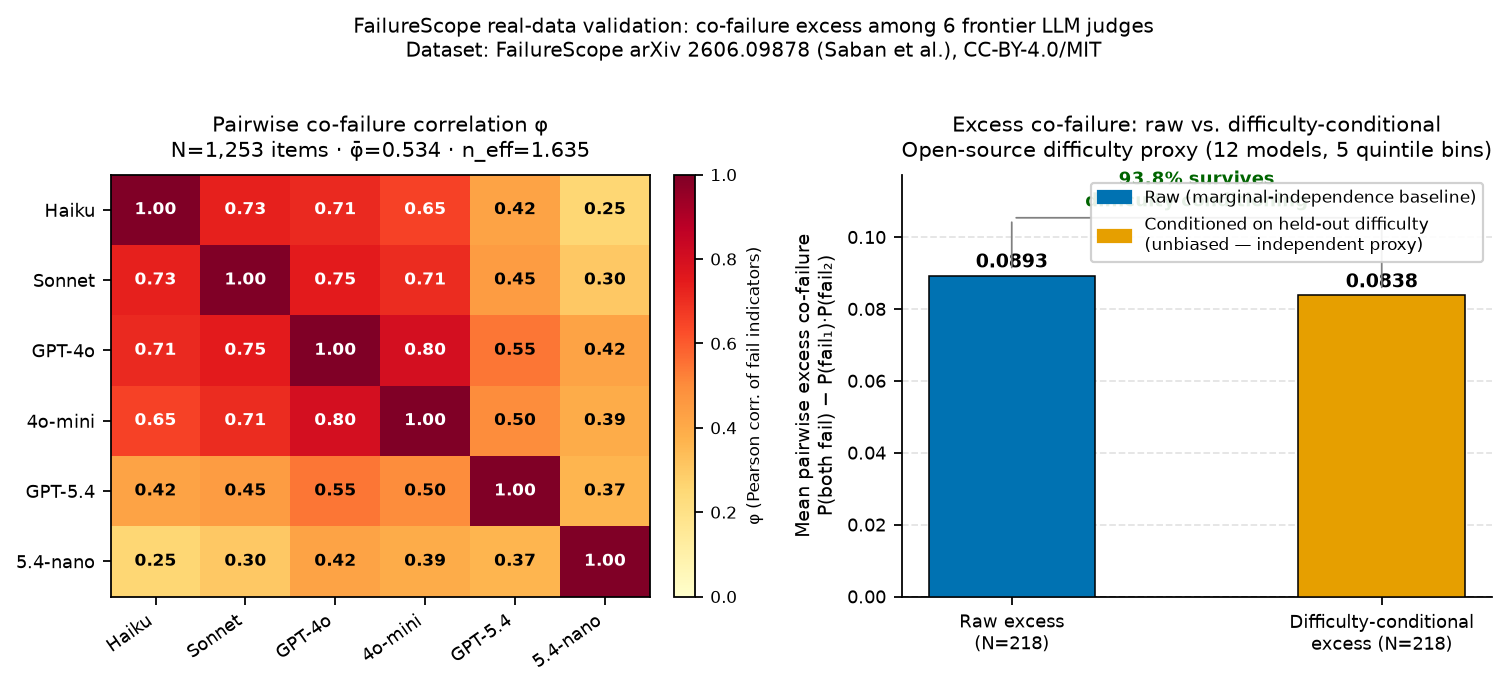
\includegraphics[width=\textwidth]{failurescope_real.png}
  \caption{Real-data co-failure on FailureScope. (Left) $6\times6$ pairwise
  co-failure correlation $\varphi$ matrix on 1{,}253 FailureScope items;
  $\bar\varphi=0.534$, $n_{\mathrm{eff}}=1.635$. (Right) Mean pairwise excess
  co-failure --- raw ($0.089$) vs.\ difficulty-conditional ($0.084$) on the
  218-item held-out subset; 93.8\% of the raw excess survives conditioning on an
  independent open-source difficulty proxy.}
  \label{fig:failurescope}
\end{figure}

\section{Power-vs-$Q$ sweep}
\label{app:qsweep}

Method A (fresh-pair within-block, quadratic slack $\delta_k=2\varepsilon_k^2$)
with $\lambda$-mixture over $\{0.1, \ldots, 0.9\}$. $Q$ = number of
equal-width strata in $\theta$. Primary metric: power at $\gamma=0.10$
common-shock probability. $N=2000$ items.

\begin{table}[h]
  \centering
  \caption{$\lambda$-mixture power sweep, $\gamma=0.10$, under the anytime-valid
  fresh-pair within-block construction. $\bar\varepsilon$ is the mean
  within-stratum half-range of $p$; the slack is quadratic
  ($\delta=2\bar\varepsilon^2$). ``Ratio'' is design slack over realised bias.
  Type-I stays $\le 0.010$ across the full sweep; power \emph{falls} as $Q$
  grows because finer stratification starves the within-block pairs. The knee is
  $Q=5$.}
  \label{tab:power}
  \small
  \begin{tabular}{@{}rrrrrrr@{}}
    \toprule
    $Q$ & $N/Q$ & $\bar\varepsilon$ & $\delta=2\bar\varepsilon^2$ & realised bias & ratio & Power ($\gamma=0.10$) \\
    \midrule
    5  & 400 & 0.050 & \textbf{0.00500} & $8.5\times10^{-4}$ & $5.85\times$ & \textbf{0.922} \\
    10 & 200 & 0.025 & 0.00125 & $8.9\times10^{-4}$ & $1.40\times$ & 0.924 \\
    20 & 100 & 0.0125 & 0.00031 & $1.5\times10^{-3}$ & $0.21\times$ & 0.814 \\
    40 & 50  & 0.00625 & 0.00008 & $2.8\times10^{-3}$ & $0.03\times$ & 0.556 \\
    80 & 25  & 0.00312 & 0.00002 & $6.2\times10^{-3}$ & $0.00\times$ & 0.264 \\
    \bottomrule
  \end{tabular}
\end{table}

Type-I stays $\le 0.010$ across the full sweep---validity never degrades as
strata become finer. The knee is $Q=5$: it already achieves power $0.922$ at
$\gamma=0.10$ with Type-I $0.010$.

\paragraph{Fixed $\lambda=0.5$ vs.\ mixture.}
The $\lambda$-mixture is load-bearing, not cosmetic: it detects a broader class
of common-shock magnitudes by hedging over unknown $\gamma$ rather than betting a
single mis-specified operating point. A clean control is the fixed-design power
at $\gamma=0.06$: with the correct quadratic slack it is restored to $0.526$,
whereas the old linear slack $\delta=2\varepsilon$ killed all power ($0.000$).
The linear slack was valid but loose by a factor $1/\varepsilon$, so at coarse
$Q$ it drowned every bet.

\paragraph{Fresh-pair starvation: the true cost of anytime validity.}
Under the genuine fresh-pair within-block construction, power \emph{falls} with
$Q$ (from $0.922$ at $Q=5$ to $0.264$ at $Q=80$). The mechanism is a design
tradeoff between stratification granularity and within-block pair availability:
at high $Q$ most (block, stratum) cells contain only a single item, which can
form no fresh same-stratum pair and therefore places no bet, starving the
e-process. The earlier whole-stream derangement masked this by pairing across the
entire stream---but that pairing reuses draws across blocks and is \emph{not}
anytime-valid (Type-I $\to 1$). The quadratic slack ratio (design slack over
realised bias) also crosses $1$ near $Q=10$: for $Q\le 10$ the slack is
conservative; for $Q\ge 20$ it is below the realised bias and the dominant loss
is pair starvation, not slack. This is the honest cost of insisting on a genuine
anytime-valid construction, not a defect: the knee sits at coarse stratification
($Q=5$), where pairs are plentiful.

\section{Extended related work}
\label{app:related}

\paragraph{Batch co-failure monitors (the lower bracket).}
Kuai et al.\ \citep{kuai2604}: same conditional-independence-given-difficulty
null, real panels, batch permutation, no Ville guarantee. Closest competitor; our
contribution is the anytime layer above it. Ming, Ramdas, Shen, Wang,
Waudby-Smith \citep{ming2603}: demi-supermartingale combiner for simultaneous
e-variables --- fixed-$n$ batch (indexed over polynomial degree, not time);
dominates sup-over-$\lambda$ averaging; cite for the co-validity condition (Def
3.1). NOT an anytime alternative for our merge step. Han \citep{han2607}: de
Finetti cascade gives a fixed-sample blind-spot ceiling $-\ln(1-\pi)$; batch;
motivates the sequential gap we fill.

\paragraph{Single-stream anytime monitors (wrong object --- marginal drift, not
co-failure).}
SKCI (He \& Sutherland, \citep{he2606}): anytime-valid conditional-independence
test via adaptive betting; single-stream; no joint co-failure null. CELEUS
\citep{celeus2606}: anytime e-process for single-model mean risk; not
co-failure. Saha-Ramdas \citep{saharamdas2607}: single-stream changepoint;
REGROW indexing; no dependence detection. Hsu \& Shekhar \citep{hsu2607}:
anytime-valid CS for mean accuracy of one LLM; no joint judge null.

\paragraph{Difficulty-confound literature.}
Jo, Garg \& Raghavan \citep{jo2602}: difficulty confound substantially attenuates
apparent co-failure correlation; proposes parametric IRT-1 null; motivates our
stratified construction as a nonparametric alternative.

\paragraph{The empty cell (our contribution):}
anytime-valid $\times$ cross-item $\times$ margins-free. Nothing in the
related-work table sits in all three.

% [One row Claudius may want to add: Wang \& Zhong \citep{wangzhong2608}
%  "N x N E-valuation" Prop 3 (means of e-values under arbitrary dependence) ---
%  anytime vs batch gate still open as of 08-17; insert if gated.]

\section{Expanded limitations}
\label{app:limitations}

\begin{enumerate}
  \item \textbf{Small-$\gamma$ gap.} Small-atom common-shock co-failure is hard:
  at $\gamma=0.04$ power is $\approx 0.07$, rising to $\approx 0.53$ at
  $\gamma=0.06$ (control sweep, $Q=10$, $N=4000$, quadratic slack). Longer
  streams or adaptive $\delta$ needed; state plainly.
  \item \textbf{Fresh-pair starvation / $Q$ as hyperparameter.} The analyst
  chooses $Q$; there is no data-adaptive procedure for $Q$ selection here. Under
  the anytime-valid fresh-pair within-block construction $Q$ is a genuine
  tradeoff dial, not merely a nuisance: finer stratification tightens the
  quadratic slack but starves the within-block pairs (singleton (block, stratum)
  cells place no bet), so power falls with $Q$ (from $0.922$ at $Q=5$ to $0.264$
  at $Q=80$). The knee is coarse stratification ($Q=5$).
  \item \textbf{$m=2$ scope.} All results are for a two-judge pair. Extension to
  $m>2$ via pairwise aggregation is natural (all pairs are valid e-processes) but
  aggregation power and control need separate treatment.
  \item \textbf{Fresh-pair within-block schedule.} Anytime validity requires the
  partner $t$ to be a \emph{fresh} same-block, same-stratum item, so that the
  partner draw is independent of the same-item draw it is compared against. The
  deprecated whole-stream derangement (pairing across the entire stream) reuses
  draws across blocks and inflates Type-I to $1$; it must not be used. The cost
  of the valid within-block schedule is pair starvation at fine $Q$ (above).
  \item \textbf{Mean vs.\ exceedance design effect.} $n_{\mathrm{eff}} = 2.18$
  (Kohli~\citep{kohli2605}) is a mean design effect; the effective size for
  vote-threshold (exceedance) decisions may differ \citep{noonan2608}.
  Our monitoring target is the mean co-failure rate, so the mean figure is
  the appropriate object here.
  \item \textbf{Single-pass filtration (no verdict leakage).} The cross-item
  pairing $V_s = W_i^s \cdot W_j^{t(s)}$ with distinct items $i \ne j$ delivers
  the margins-free independence baseline $\mathbb{E}[V_s]=p_i p_j$ that the
  co-failure e-process relies on \emph{only} under single-pass evaluation. In a
  multi-round orchestration that passes prior verdicts between rounds or between
  judges, this independence can break: a leaked prior verdict contaminates the
  filtration to which the e-process is adapted---the data-pipeline analogue of
  briefing a verifier with the very conclusion it is meant to check
  independently. The anytime validity is therefore \emph{conditional} on a
  deployment requirement: the orchestration must not leak prior verdicts into
  the filtration that the cross-item e-process is adapted to. We state this as
  an explicit scope condition, not a property that holds automatically.
\end{enumerate}

\end{document}
